\documentclass[11pt]{article}
\usepackage[a4paper,margin=25mm]{geometry}
\usepackage{amsmath,amssymb,amsthm,booktabs,tabularx,array,enumitem,graphicx}
\usepackage[colorlinks=true,allcolors=blue]{hyperref}
\emergencystretch=3em
\newcommand{\R}{\mathbb{R}}
\newcommand{\TE}{\operatorname{TE}}
\newcommand{\SIZE}{\operatorname{SIZE}}
\renewcommand{\thetable}{S\arabic{table}}
\newtheorem{proposition}{Proposition}
\title{Execution-Constrained Portfolio Rebalancing: Policy Domains, Search and Numerical Reliability\\Supplement: formulation, replication and difficulty results}
\author{Artur Sepp\\LGT}
\date{}
\begin{document}
\maketitle

This supplement specifies the methods evaluated with OptimalPortfolios 9.2.0.
``Exact Execution'' denotes the matched joint solver and ``Ranked Execution''
the ranked search, historically implemented in \texttt{execution/v2}.
Method names do not change the identity of the evaluated software. The older
operational MIQP implementation has a different policy and is not the matched
comparator. This document adds no production rule or numerical tolerance.

\section{Declared state domain and formulation}
Let $c,m,w\in\R^N$ denote original current, raw target and final weights;
$k$ denotes settlement cash. All weights are fractions of net asset value.
Table~\ref{tab:notation} collects the principal symbols.
\begin{table}[htbp]\centering\small
\caption{Notation and distinct numerical conventions.}\label{tab:notation}
\begin{tabularx}{\linewidth}{lX}\toprule
Symbol & Meaning\\\midrule
$c,m,w$ & Original current, raw target and delivered weight vectors.\\
$q,r$ & Common prepared base and the funded reference used in coordinate elimination.\\
$N,k$ & Number of coordinates including cash, and settlement-cash index.\\
$\Sigma,f,\TE$ & Annual covariance, tracking variance and its square root.\\
$L,U,a,A,b$ & Hard instrument bounds and fractional group-exposure rows.\\
$\ell_{ij},u_{ij},t_{ij}$ & State endpoints and its noncash ticket label.\\
$\delta_i,\theta_i$ & Minimum delivered trade and minimum positive holding.\\
$M,B,K$ & Reserved mandatory names, optional allowance and total ticket capacity.\\
$10^{-8},10^{-7}$ & Trade-zero threshold and portfolio audit tolerance, in NAV fractions.\\
$\epsilon=10^{-12}$ & Search improvement/comparison scale, in annual variance.\\
$10^{-4}$ bp & Descriptive TE equality band, distinct from audit acceptance.\\
\bottomrule\end{tabularx}\end{table}
For each noncash instrument $i$, let $J_i$ be a finite set of labelled closed
intervals. State $j$ has endpoints $\ell_{ij},u_{ij}$ and ticket label
$t_{ij}\in\{0,1\}$. State construction intersects the permitted movement with
the hard instrument bounds, minimum trade and zero-or-minimum-holding rules.
The nominal no-trade state is $[c_i,c_i]$ with label zero. Ordinary buy and
sell states exclude nonzero movements smaller than the minimum ticket.
An eligible full exit may be a separate state.

Mandatory declarations are resolved before search. Their admissible intervals
exclude the original holding and have ticket label one. An explicit minimum
ticket exemption changes the minimum-size rule only; it does not remove the
ticket or the holding floor. The compulsory interval need not be a singleton.
Let $I_O$ be the optional instruments and let $K,B$ be the total and optional
ticket capacities, when specified. The state domain consists of an admissible
labelled interval choice for every noncash instrument, together with
\begin{equation}\label{eq:hard}
 \mathbf 1^\top w=1,\qquad L\le w\le U,\qquad a\le Aw\le b,
\end{equation}
and the declared ticket sums. Cash has no ticket and remains bounded.

\begin{proposition}[Interval-state formulation]
Introduce binary selectors $z_{ij}$ and contributions $v_{ij}$ satisfying
\begin{align}
 \sum_{j\in J_i}z_{ij}&=1,&
 \ell_{ij}z_{ij}\le v_{ij}&\le u_{ij}z_{ij},&
 w_i&=\sum_{j\in J_i}v_{ij},\label{eq:states}\\
 \sum_{i\ne k}\sum_{j\in J_i}t_{ij}z_{ij}&\le K,&
 \sum_{i\in I_O}\sum_{j\in J_i}t_{ij}z_{ij}&\le B.\label{eq:counts}
\end{align}
Omit a capacity row when that capacity is unspecified. Together with
\eqref{eq:hard}, the integer formulation projects exactly onto the declared
labelled state domain.
\end{proposition}
\begin{proof}
For each instrument, exactly one selector is one. All other contributions
are zero by their two bounds. The remaining contribution is the final weight
and lies in its chosen interval. The corresponding labels give precisely
the two ticket sums. Conversely, select the declared state of every admissible
portfolio, assign its weight to that state's contribution and set all other
contributions to zero. Equations \eqref{eq:states}--\eqref{eq:counts} and the
unchanged hard rows hold. Cash is determined by funding and retains its bounds.
\end{proof}

This is an application of a standard disjunctive extended formulation;
see Vielma (2015), Section 5. It is not a claim that the continuous relaxation
of the coupled portfolio problem is ideal. Ideal formulations of individual
sets need not describe the convex hull after additional coupling constraints.

\paragraph{Mathematical domain and numerical audit.}
The proposition concerns the specified intervals and linear rows. Released
code permits numerical base-current differences up to the trade-zero threshold
and compiles a group residual envelope at the existing audit tolerance.
Consequently the proposition is not an equivalence between an exact symbolic
domain and every vector that a finite-precision audit may accept. Every
candidate is checked against the original supplied inputs. The study keeps
audit tolerance $10^{-7}$ NAV and trade-zero tolerance $10^{-8}$ unchanged.
The descriptive TE equality band $10^{-4}$ annual bp is not a feasibility
tolerance. Search improvement uses $10^{-12}$ annual variance.

\subsection{Funding elimination and objective origin}
Fix coordinates that cannot move. Choose a funded reference $r$ and let $D$
contain one column $e_i-e_k$ for every remaining noncash coordinate. Every
funded vector with those fixed coordinates has the unique representation
$w=r+Dx$, where $x_i=w_i-r_i$. Substitute this expression into all bounds and
group rows, including cash bounds. With $\Sigma\succeq0$ annual covariance,
\begin{equation}\label{eq:funded}
 f(r+Dx)=x^\top Qx+2g^\top x+f(r),\quad
 Q=D^\top\Sigma D,\quad g=D^\top\Sigma(r-m).
\end{equation}
For every $x$, $x^\top Qx=(Dx)^\top\Sigma(Dx)\ge0$, so $Q$ is positive
semidefinite. This is exact funding substitution, not a diagonal approximation.

Multiplication by a positive scalar preserves the mathematical minimiser.
Removing $f(r)$ also preserves that minimiser but changes the objective origin
seen by a relative stopping rule. Restore both scale and constant when reporting
an incumbent or bound. Compare a solver's native bound with a delivered,
independently audited incumbent in original variance units. The best native
incumbent may itself fail the audit; its native gap can then be smaller than
the delivered portfolio's gap. Restricted Kernel Search bounds are not global
bounds for the full execution problem.

\subsection{Perspective guidance}
Choose a nonnegative diagonal matrix $\operatorname{diag}(d)$ such that
$Q_0=Q-\operatorname{diag}(d)\succeq0$. Let $y_i$ be optional ticket occupancy;
use $y_i=1$ for mandatory coordinates. The no-ticket state fixes $x_i=0$.
The perspective objective in unscaled funded coordinates is
\[
 f(r)+2g^\top x+x^\top Q_0x+\sum_i d_i\,\psi(x_i,y_i),\qquad
 \psi(x,y)=\begin{cases}x^2/y&y>0,\\0&x=y=0,\\+\infty&y=0,\ x\ne0.\end{cases}
\]
Each perspective term is convex. At integer occupancy it equals $x_i^2$ on
every admissible state, preserving the original objective. For $0<y_i\le1$
it is at least $x_i^2$, so it strengthens the ordinary continuous objective
on the same relaxed state rows. The resulting optimal relaxation value is
a lower bound on the integer optimum. These are standard perspective
properties (Frangioni and Gentile, 2006; G\"unl\"uk and Linderoth, 2010).

Released guidance uses a conservative verified diagonal split, not an
optimised diagonal decomposition; a zero split gives no strengthening.
An approximate conic primal value is not automatically a lower bound.
The separate OP bound routine constructs a supporting plane and minimises it
over the linear relaxation, with an LP dual residual correction on bounded
variables. This certificate route is separate from native mixed-integer bound
diagnostics. The prospective Exact arms retain the released non-perspective
default; Kernel and Ranked use perspective guidance for priorities. The study
therefore evaluates those declared implementations, not the strongest possible
mixed-integer formulation.

\subsection{A corridor counterexample}
Let
\[
 c=(0.2,0.2,0.6),\quad m=(0.3,0.3,0.4),\quad
 \Sigma=0.01\begin{pmatrix}1&0.9&0\\0.9&1&0\\0&0&0\end{pmatrix},
\]
with cash last, hard bounds $[0,1]$, one noncash ticket, no mandatory action,
minimum trade $0.005$ and holding floor $0.0025$. The ordinary risky corridors
are $[0.2,0.3]$ and cash remains in $[0,1]$.
If the first instrument trades, the second remains at $0.2$. Writing
$x=w_1-0.3$ gives
\[
 f(w)=0.01(x^2-0.18x+0.01).
\]
The unrestricted minimum is at $x=0.09$, giving $w=(0.39,0.2,0.41)$,
variance $0.000019$ and TE $43.5889894354$ annual bp. In the corridor,
$x\in[-0.1,0]$ and the minimum is at zero, giving $w=(0.3,0.2,0.5)$,
variance $0.0001$ and TE $100$ bp. Trading the second instrument gives the
symmetric solutions; no trade is worse. These scalar cases exhaust the ticket
choices independently of either execution algorithm.

The overshoot offsets an untraded correlated underweight. Thus a corridor is
an economic policy restriction, not a generally lossless reduction of the
full hard domain. The replication test checks the scalar objectives and both
solver domains without changing either audit tolerance. Comparisons of
time-limited Full and Corridor incumbents do not by themselves measure the
optimal restriction cost: their search errors can differ.

\section{Ranked Execution: ordered specification}
A support $S$ maps selected optional instruments to executable state indices.
Mandatory state assignments are separate. The released defaults are rescue
budget $R=24$, mandatory-assignment budget $H=32$, improvement-pass budget
$P=3$ and variance-improvement threshold $\epsilon=10^{-12}$.
Identifier and then state index resolve priority ties. A returned incumbent
must pass the original-input audit; a relaxed or tentative vector never serves
as a delivery solely because it produced a promising priority.

\subsection{Sizing and common state}
Maintain a support cache keyed by sorted $(i,j)$ pairs. For a previously unseen
support, $\SIZE(S)$ first checks capacity, then tries at most $H$ mandatory
assignments in distance-from-base and state-index order. Pin unselected
optional names to their no-ticket states and jointly size all selected names
with the common convex quadratic model and unchanged hard rows. Audit each
candidate and cache the best accepted result, or the attempted failure.
Different search branches have separate visited sets but share this cache.
A failed sizing attempt is not a proof that the state assignment is infeasible.
Candidate acceptance requires an improvement greater than $\epsilon$.

The funded scalar priority for an optional movement $d$ in name $i$ is
\[
 f(w+d(e_i-e_k))-f(w)
 =2d(e_i-e_k)^\top\Sigma(w-m)
  +d^2(e_i-e_k)^\top\Sigma(e_i-e_k).
\]
Minimise this quadratic over the state's movement interval; for two-name
priorities retain the cross term between their funded directions. A priority
does not replace the subsequent joint sizing or audit.

\subsection{Search order}
The following order matters because later seeds, caches and incumbents depend
on earlier accepted results.
\begin{enumerate}[leftmargin=*,itemsep=0.45em]
\item Compile states, retain the audited prepared base and determine optional
capacity. If the declared state domain conflicts with capacity, retain an
audited base if available. Enumerate the bounded mandatory assignments once.
\item From the base, greedily add distinct optional names using the funded
scalar priorities. Update the covariance product after each tentative move.
Stop at capacity or when no scalar gain remains.
\item Size the empty support when mandatory intervals can move, then the greedy
support. For failed sizing, try up to $R$ drop, admission, state-change or
replacement rescue supports ordered by coupled group pressure and identifier.
\item Run single-drop and best-ranked replacement passes. Run up to $P$
coordinated anchors sharing $R$ shortlisted support trials. Initial coordinated
moves edit one or two instrument states and use conditional funded quadratics.
\item When capacity is positive and below the candidate count, solve the
unrestricted perspective guidance relaxation. Select at most capacity names
by fractional occupancy, with their largest eligible state selectors. Explore
this seed separately while preserving the global incumbent. Run expanded
coordinated improvement, complete single-replacement sweeps and up to $R$
shared coordinated trials, including the guidance seed.
\item Restart from the completed incumbent and a distinct unrestricted guided
seed. Exclude each of up to $R$ incumbent names in separate guidance problems.
Give every distinct seed at most $P$ complete one-for-one replacement sweeps.
An inferior audited seed may initiate a branch, but only its completed
improvement may replace the global incumbent. Failed rounded seeds may receive
a one-swap rescue.
\item Form the identifier-ordered union of incumbent and unrestricted-guidance
states. Try inclusion then exclusion, up to $R$ conditional guidance calls.
Guidance changes the seed only: sizing always uses the unmodified problem.
Restart distinct seeds and revisit the completed conditional incumbent.
\item Complete up to $P$ expanded anchors sharing $R^2$ coordinated trials,
skipping cached supports. Expanded moves include two admissions with one or
two removals. Apply a necessary interval-envelope funding and group screen
before sizing. Each anchor also performs a complete replacement sweep.
\item Sort cached audited alternatives by objective and identifier and restart
at most $R$. The first branch improving the global incumbent receives one
further $P$-anchor, $R^2$-trial completion. Return the best audited incumbent
with truncation and failure diagnostics.
\end{enumerate}

An \emph{anchor} is the incumbent support at the start of an improvement pass.
\emph{Rescue} seeks feasible sizing after a tentative support fails.
A \emph{shortlist} limits supports sent to sizing after priority enumeration.
\emph{Completion} denotes a finite extra neighbourhood budget, not exhaustive
search. A bridge restart starts from a cached alternative while preserving
the best incumbent in separate state. None of these stopping conditions
certifies global optimality.

\subsection{Computational scope}
Let $C$ be eligible optional names, $S_t$ ticket states, $B$ capacity, $G$ group
rows and $T$ distinct supports submitted to sizing. At most $HT$ fixed-state
QPs are attempted, in addition to guidance solves. A complete replacement
sweep examines order $BS_t$ proposals. Two admissions with up to two removals
can generate order $(B+B^2)S_t^2$ proposals per anchor before the bounded
shortlist. Screens add dependence on $G$ and some full-vector work. A bounded
sizing budget therefore does not establish an $O(NB)$ runtime or a small
wall-clock bound.

An exact factor-plus-diagonal covariance with $r$ factors uses order
$Nr+r^2+N$ input storage. The released implementation nevertheless constructs
a dense $N\times d$ funded map and a dense $d\times d$ funded Hessian, where
$d$ counts unfixed noncash coordinates. Mandatory intervals can contribute
to $d$. QIS reporting also materialises the $N\times N$ covariance. Reported
peak worker memory includes imports and reporting; it is not a measurement
of only the branch-and-bound model. Structured input does not establish
linear-memory execution.

\section{Kernel Search comparison}
The comparator adapts the restricted-kernel and bucket scheme in Guastaroba
and Speranza (2012, 2014) to the same convex quadratic execution states. It
does not reproduce their index-tracking MILP. It ranks names by fractional
ticket occupancy from the perspective relaxation, rather than LP reduced
costs. The initial kernel has $\min(C,\max(24,2B))$ names, with stable
identifier ties. Divide the remaining ordered names into disjoint buckets
of that initial size.

First solve on the kernel, then make one pass through kernel-plus-bucket
subproblems. Pin excluded optional names to the prepared base. Retain every
mandatory state and all original hard rows. Each bucket subproblem requires
at least one bucket ticket and has an incumbent cutoff of best variance plus
$10^{-12}$. Divide the remaining internal allowance among remaining stages.
Names selected by an audited bucket solution join the kernel. There is no
ageing, removal or later refinement. The common prepared base supplies a
feasible initial candidate when it passes audit; no incumbent is imported
from another comparison arm.

The 60-second allowance includes guidance, model construction and subproblem
search. Independently audit both original and restricted domains and verify
bucket use before retention. Restricted-subproblem bounds cannot certify
the unrestricted problem. The adaptation is a literature-based control with
declared choices, not a claim of the best attainable Kernel Search tuning.

\section{Prospective difficulty protocol}
The machine-readable authority is \texttt{study\_protocol.json}. Before any
evaluation solve, the runner freezes all cases, source bytes, wheel identity,
ordering, versions and resource limits. The retained earlier 313 cases and
the four resource-planning pilot cases remain separate from this evaluation.
No solver is modified after inspecting this cohort.

\subsection{Sparse synthetic books}
There are 18 scaling cases: 300, 1,000 or 3,000 noncash universe names;
10, 30 or 100 optional tickets; and two bundled profiles. Current holdings
use 96 names, each at least 0.6\%, with 6\% settlement cash. Targets add 100
names and hold 2\% cash. The 0.5\% minimum ticket and 0.25\% holding floor are
fixed. Universe size, held positions and executable candidates are distinct:
the wide cells have 155 eligible optional names and the tight cells have 190.
The number of ticket states ranges from 200 to 280 across these cells.

The wide profile combines disjoint groups, diffuse target support and two
mandatory exits. The tight profile combines overlapping fractional rows,
exit-rich targets and six mandatory exits. Each profile has one predeclared
seed, shared across its size and capacity cells. Risk uses exactly twelve
factors plus diagonal residual variance. Separate random streams construct
current holdings, target and risk; streams also depend on universe size.
Within a size/profile cell, changing ticket capacity preserves those inputs.
Cross-size differences therefore include different random books and cannot
isolate a pure universe-size effect. Profiles bundle multiple features and
differ in seed: their contrast is not a factorial estimate or population
superiority claim. An independently audited base witnesses feasibility.

\subsection{External covariance adaptation}
Four further cases use the OR-Library \texttt{indtrack1} and
\texttt{indtrack6} price panels, with 31 and 457 stocks, at observation cuts
145 and 290. Holdings, targets, cash and every execution constraint remain
synthetic. The source format provides price observations without calendar
dates. Artificial weekly labels and 52 periods per year are explicit model
conventions, not recovered historical dates or frequencies.

QIS computes point-in-time demeaned log-return EWMA covariance with span 52,
using only prices through the cut. Annualisation multiplies the period
covariance by 52. Synthetic cash variance is $10^{-6}$. The source index
series is not used as the execution target. These are externally sourced
risk cases, not replications of the original index-tracking objective.
Public code records owner URLs, source checksums and transformation. Raw
price files and their derived covariance arrays are excluded from the
redistribution archive pending established reuse terms; fetch from the owner
to reproduce locally.

\subsection{Accounting and denominators}
The 23 cases comprise the 18 scaling cells, four external-risk cases and the
analytic counterexample. Each has independent Exact60, Ranked and Kernel60
arms. Each tight, 30-ticket scaling cell additionally has Exact10, Exact600,
Dense10 and Full60; the counterexample also has Full60. This totals 82
planned deliveries. Dense10 changes covariance representation only; Full60
changes the corridor policy domain while preserving common preparation and
hard rows.

Cases run serially with one solver and numerical-library thread. Arm order
rotates by case index, each in a fresh process. Preparation has a 30-second
internal allowance and a 90-second process ceiling. Exact10, Exact60 and
Exact600 receive 10, 60 and 600 seconds, with process ceilings 60, 120 and
660 seconds. Kernel60, Dense10 and Full60 have 120-second process ceilings.
Ranked retains its released stopping controls with a 180-second external
process ceiling; this does not add a new internal stopping algorithm.

Charge common preparation to every arm, time covariance conversion separately,
and record engine, end-to-end worker and complete process times. A killed
worker without a delivered result remains a failed delivery, even if it had
an internal incumbent. Preserve any boundary result separately. Timing
summaries include failures where a process duration exists; missing memory
measurements are not invented. Paired TE comparisons state the number of
audited pairs and the number missing. Native statuses and bounds, audit
acceptance and independently proved optimality remain separate evidence.

The supplied prepared base is already feasible. Time to the first audited native
candidate can therefore measure acceptance of that lifted start rather than
discovery of an improvement. Kernel likewise records initial feasibility at
zero when the base passes audit. Ranked has no new anytime-delivery interface
in this study: a process ceiling means that no portfolio was returned by that
deadline, not that the search never held a feasible internal incumbent. The
different declared resource controls compare these released interfaces; they
are not a matched wall-clock anytime experiment.

Source and input identity do not imply identical time-limited search paths on
different hosts or reruns. A wall-clock cutoff can stop at a different incumbent.
The resource protocol, all failed attempts and original-input audits are part
of reproduction; the retained run provides the exact observations used here.

\section{Isolated numerical mechanism controls}
These controls use retained public regression examples, separately from the
prospective instances. They change equivalent graph representations in an
isolated research process; installed package files and production settings
remain unchanged. Their purpose is to expose mechanisms and their limits,
not to provide additional out-of-sample success counts.

\paragraph{Objective translation.}
For an incumbent value $F_U$, lower bound $F_L$ and positive scale $\alpha$, translation
to $\alpha f+\beta$ leaves the mathematical minimiser unchanged but changes
the relative gap, with denominator floor $\eta>0$, to
\[
 \frac{\alpha|F_U-F_L|}{\max(\eta,|\alpha F_U+\beta|)}.
\]
Take $F_U=10^{-10}$, $F_L=9\times10^{-11}$ and remove a constant $10^{-3}$.
The original relative gap is $0.1$; the translated gap is approximately
$10^{-8}$. The absolute gap $10^{-11}$ exceeds the unchanged $10^{-12}$
variance allowance. Thus a $10^{-4}$ relative criterion can accept the
translated pair while rejecting the original pair. This is an analytical
bound-pair example, not fabricated native solver output.

\paragraph{Equivalent quadratic cones.}
Use the same public 24- and 72-optional-name examples and the same state rows.
Compare $x^\top Qx/10^4$ with $(x/100)^\top Q(x/100)$, where $x$ is funded
displacement in basis points. Retain the linear term, constant and original
variance origin in both graphs. Both variants receive ten seconds, one native
thread and the released numerical settings. Every returned candidate passes
through the same original-input audit before it may displace the prepared base.
For the 24-name example an independent full-weight reference on a known support
provides a feasible witness. It is not automatically a global certificate for
the 72-name problem. A control that does not reproduce a prior defect under
this runtime is reported as such.

\paragraph{Satisfied constant rows.}
After fixed-coordinate elimination, a group exposure can become constant.
The released sizing compiler removes a row only when its coefficients are
exactly zero and its constant satisfies both compiled endpoints. It retains
every nonconstant row and every constant contradiction. The control compares
retaining versus removing satisfied rows, for both a lower and an upper
fractional-exposure limit. Residuals are $(1-10^{-8})\times10^{-7}$ and
$1.01\times10^{-7}$ NAV, respectively inside and outside the unchanged audit
envelope. This gives eight graph variants. The feasible cases are checked
against an independent active-set calculation after removing the mathematically
redundant row; the outside-envelope cases have an immediate constant-row
infeasibility witness. Native status, errors and audited delivery are retained
separately. Removing a redundant row is not permission to discard a genuine
constraint breach.

\section{Completed prospective results}
All 23 cases prepare successfully and all 82 declared attempts are retained.
There are 64 audited deliveries and 18 process-ceiling failures, all from
Ranked. No returned portfolio fails the independent original-input re-audit.
Preparation recognises an already audited base in every new case; this sample
therefore does not measure the difficulty of discovering compulsory repairs.
It tests optional search conditional on the declared mandatory movements and
common feasible base.

\subsection{Delivery, quality and computation}
Exact60 and Kernel60 deliver in all 18 scaling cases. Ranked delivers in two
and reaches its 180-second process ceiling in 16. Of the two returned Ranked
portfolios, one ties Exact60 and one improves it by 2.402490 bp; both have
higher TE than Kernel60. Kernel60 improves on Exact60 in 11 cases, ties in
four and is worse in three. Its signed differences range from $-55.718876$
to $23.386397$ bp. These are comparisons of audited incumbents, not errors
relative to a proven optimum. The fixed resource controls and different
delivery interfaces are part of the comparison.

\begin{table}[htbp]\centering\small
\caption{Delivery and process cost in the prospective study. Exact and Kernel have 60-second internal allowances; Ranked retains released defaults with a 180-second process ceiling. Process time includes imports and reporting. Memory is the largest observed worker peak, with its observation count in parentheses; killed workers have no peak measurement.}\label{tab:scalingtime}
\begin{tabular}{llrrrr}\toprule
Sample & Method & Audited & Median s & 95th pct. s & Observed MiB\\\midrule
Scaling & Exact & 18/18 & 66.312 & 67.411 & 746.137 (18)\\
Scaling & Ranked & 2/18 & 180.019 & 180.026 & 497.750 (2)\\
Scaling & Kernel & 18/18 & 66.647 & 67.823 & 762.730 (18)\\
External risk & Exact & 4/4 & 35.760 & 65.471 & 321.340 (4)\\
External risk & Ranked & 2/4 & 99.137 & 180.021 & 271.801 (2)\\
External risk & Kernel & 4/4 & 35.840 & 66.089 & 348.336 (4)\\
\bottomrule\end{tabular}\end{table}
\begin{table}[htbp]\centering\small
\caption{Paired audited TE differences, left method minus Exact60, in annual bp. Negative differences favour the left method. Open Exact gaps mean these are incumbent comparisons. The equality band is $10^{-4}$ bp.}\label{tab:scalingquality}
\begin{tabular}{llrrrrrr}\toprule
Sample & Left & Paired & Lower & Ties & Higher & Min bp & Max bp\\\midrule
Scaling & Ranked & 2/18 & 1 & 1 & 0 & -2.402 & 0.000\\
Scaling & Kernel & 18/18 & 11 & 4 & 3 & -55.719 & 23.386\\
External risk & Ranked & 2/4 & 0 & 2 & 0 & 0.000 & 0.000\\
External risk & Kernel & 4/4 & 0 & 2 & 2 & 0.000 & 0.361\\
\bottomrule\end{tabular}\end{table}


The four external-risk cases give a different result. Exact60 and Kernel60
both deliver four portfolios. They tie on the two 31-name cases; Exact has
lower TE on the two 457-name cases, by 0.191694 and 0.361215 bp. Ranked ties
Exact on the two smaller cases and returns no portfolio by its deadline on
the two larger ones. Neither the scaling nor external sample supports an
unconditional ranking of algorithm families.

The optional ticket cap binds in ten of 18 scaling Exact60 deliveries and
12 of 18 Kernel60 deliveries. The two completed scaling Ranked calls use
zero and two optional tickets. Current holdings, target support and executable
candidate counts are distinct from the nominal universe. In particular,
increasing the universe to 3,000 does not create 3,000 Corridor candidates.

Table~\ref{tab:scalingtime} reports complete method-process duration, including
imports and reporting, and keeps killed calls in the timing denominator.
Adding each common preparation process gives scaling median research-pipeline
times of 72.871 seconds for Exact, 186.578 for Ranked and 73.245 for Kernel.
These research-process figures include two import phases; they are not direct
predictions for a persistent production process. The largest observed worker
peaks are approximately 746 MiB for Exact and 763 MiB for Kernel. The worker
includes dense QIS risk reporting. Missing killed-worker memory measurements
do not imply low memory consumption by Ranked.

\begin{figure}[htbp]\centering
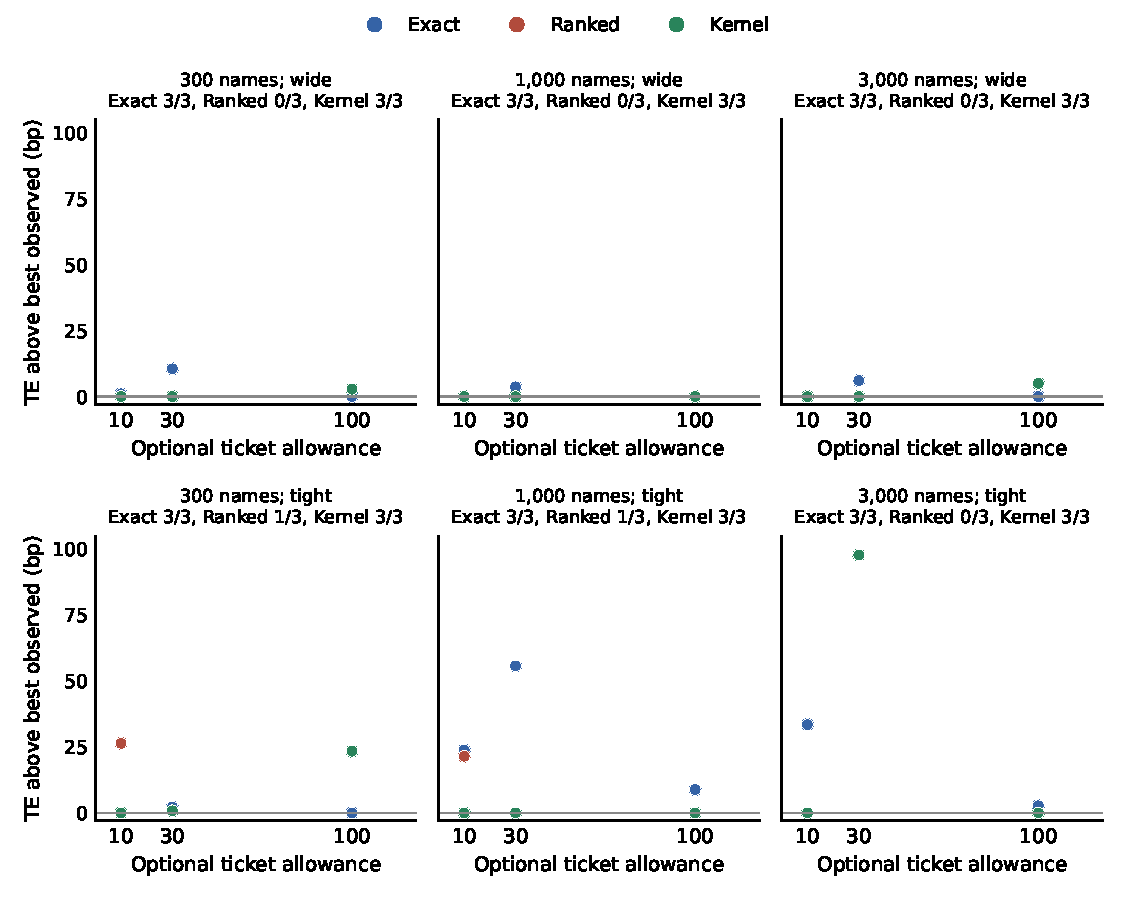
\includegraphics[width=\linewidth]{figures/difficulty_comparison.pdf}
\caption{Audited TE above the best observed Corridor delivery in each scaling
case. The reference includes Exact600 where it was prespecified. Full-domain
portfolios are excluded. Panel counts retain missing deliveries; no point is
imputed for a process ceiling. Zero means agreement with an observed incumbent,
not a certificate of optimality.}\label{fig:difficulty}
\end{figure}

\subsection{Longer budgets, domains and native diagnostics}
Only two of the 18 scaling Exact60 calls report native integer-optimal status;
the other 16 report primal-feasible status. Their median native relative gap
is 15.771\%, and the maximum is 72.637\%. Two external-risk Exact60 calls
report integer-optimal status and two primal-feasible status. There is no
native-bound contradiction against an available audited witness in the same
domain at the unchanged $10^{-12}$ variance comparison scale. This check
does not independently certify an unfinished bound or optimum.

\begin{table}[htbp]\centering\small\setlength{\tabcolsep}{4pt}
\caption{All prespecified 30-ticket, tight-profile controls. TE is annual bp. Full60 changes the policy domain; its difference is not search error on the Corridor problem. The final column reports the native relative gap for Exact600, which can differ from the gap of the audited delivery.}\label{tab:studycontrols}
\begin{tabular}{rrrrrrr}\toprule
Names & Exact10 & Exact60 & Exact600 & Dense10 & Full60 & Native gap \%\\\midrule
300 & 133.627 & 92.849 & 90.613 & 133.627 & 133.627 & 7.554\\
1000 & 159.813 & 159.813 & 159.813 & 159.813 & 159.813 & 61.837\\
3000 & 210.198 & 210.198 & 112.441 & 210.198 & 210.198 & 3.170\\
\bottomrule\end{tabular}\end{table}


The three Exact600 controls remain unresolved. Increasing 60 seconds to
600 improves the 300-name case by 2.236112 bp and the 3,000-name case by
97.757191 bp. The 1,000-name case remains at its common prepared incumbent,
with native relative gap 61.837\%; Kernel60 improves that incumbent by
55.718876 bp. Native callback records for that Exact600 case contain no
rejected better vector. Its failure to improve cannot be attributed to
rejection at an audit boundary.

Across the scaling Exact60 calls, 20 native candidate events fail the audit;
these are candidate events, not 20 failed portfolio deliveries. A native
incumbent can differ from the accepted portfolio. For example, the 300-name,
ten-ticket wide case has native incumbent variance 0.000130181637 but delivers
0.000132001026 after the better native candidate exceeds the group audit
envelope. Both the native and delivered gaps are retained, and no tolerance
is widened to accept that candidate.

Dense10 and structured Exact10 return the same prepared base in all three
representation controls. This result does not show that their search paths
or memory costs are equal. Likewise all three Full60 controls return the
base: one is worse than Corridor Exact60 and two tie. Those unfinished results
cannot estimate the optimal cost of the corridor restriction. The analytic
case does establish a possible cost independently: all three Corridor methods
give 100 bp, while Full gives 43.588989 bp, matching the scalar calculation.

\subsection{Historical controls and interpretation}
The earlier 313-case cohort remains a separate immutable study. Its ETF
decisions have only zero to five effective optional candidates; its four
fresh-holdout Ranked misses and 12 economically tiny ETF advantages remain
visible in Table~\ref{tab:historical}. Its primary/fallback wrapper had zero
natural fallbacks and nine successful injected fallbacks. No wrapper was
run on the new difficulty sample, so standalone failures cannot be converted
into an observed fallback frequency.

\begin{table}[htbp]\centering\small\setlength{\tabcolsep}{4pt}
\caption{Retained 313-case cohort: Ranked minus independent Exact TE, in annual bp. Negative differences favour Ranked. The equality band is $10^{-4}$ bp; the smaller ETF differences remain visible.}\label{tab:historical}
\begin{tabular}{lrrrrrr}\toprule
Sample & Paired & Ranked lower & Ties & Ranked higher & Minimum & Maximum\\\midrule
ETF & 219 & 12 & 207 & 0 & -0.000941 & 0.000043\\
Existing synthetic & 26 & 0 & 26 & 0 & 0.000000 & 0.000000\\
Fresh holdout & 68 & 0 & 64 & 4 & 0.000000 & 2.457878\\
\bottomrule\end{tabular}\end{table}


These observations support a study of the declared execution domain, numerical
representation and measured computational limits. They do not support a claim
that Ranked is generally superior to Exact, that Exact is universally faster
or better, or that a fallback wrapper removes search risk. Kernel's advantage
is substantial in several synthetic cells but reverses in others. The
prespecified bundled profiles, limited seeds and conditional supplied-input
design do not establish population or realised investment-performance claims.
Any formulation strengthening or new stopping interface requires separate
development and another frozen evaluation.

\subsection{Numerical mechanism outcomes}
All four cone controls return audited portfolios and native integer-optimal
labels. Nevertheless the unbalanced representations report bounds above
better audited witnesses on the same inputs, by $7.630\times10^{-11}$ and
$5.439\times10^{-10}$ original variance for 24 and 72 optional names.
Both exceed the unchanged $10^{-12}$ comparison scale. The balanced variants
show no such contradiction at that scale. The resulting TE differences are
economically small; the issue is the numerical validity and attribution of
the bound. These isolated research variants do not alter released code.

\begin{table}[htbp]\centering\small
\caption{Equivalent cone controls under unchanged native settings. Variances are in original annual units. Excess is the native bound minus the best audited witness from the two equivalent graphs, in units of $10^{-12}$ variance. A native optimal label does not remove a contradictory witness.}\label{tab:numericcones}
\begin{tabular}{rlrrr}\toprule
Optional & Graph & Delivered variance & Native bound & Excess\\\midrule
24 & Unbalanced & 0.000176888072 & 0.000176888082 & 76.299\\
24 & Balanced & 0.000176888006 & 0.000176888006 & 0.000\\
72 & Unbalanced & 0.000164967505 & 0.000164967562 & 543.918\\
72 & Balanced & 0.000164967018 & 0.000164967018 & 0.000\\
\bottomrule\end{tabular}\end{table}


The constant-row controls do not reproduce the historical sizing failure in
this runtime. Both retained-row and reduced-row graphs solve the two
inside-envelope cases and agree with the independent active-set variance
0.0013375 to floating-point precision. All four outside-envelope graph
variants are infeasible. Thus these controls support preservation of genuine
breaches, but provide no measured delivery advantage for row elimination here.
The objective-translation example remains an analytical stopping-rule
counterexample, separately labelled from native observations.

\section{References}
\begin{itemize}[leftmargin=*,itemsep=0.65em]
\item Frangioni, A. and Gentile, C. (2006). Perspective cuts for a class of
convex 0--1 mixed integer programs. \emph{Mathematical Programming} 106(2),
225--236. \url{https://doi.org/10.1007/s10107-005-0594-3}.
\item G\"unl\"uk, O. and Linderoth, J. (2010). Perspective reformulations of
mixed integer nonlinear programs with indicator variables. \emph{Mathematical
Programming} 124, 183--205. \url{https://doi.org/10.1007/s10107-010-0360-z}.
\item Guastaroba, G. and Speranza, M.G. (2012). Kernel Search: An application
to the index tracking problem. \emph{European Journal of Operational Research} 217,
54--68. \url{https://doi.org/10.1016/j.ejor.2011.09.004}.
\item Guastaroba, G. and Speranza, M.G. (2014). A heuristic for BILP problems:
The Single Source Capacitated Facility Location Problem. \emph{European
Journal of Operational Research} 238, 438--450.
\url{https://doi.org/10.1016/j.ejor.2014.04.007}.
\item Vielma, J.P. (2015). Mixed integer linear programming formulation
techniques. \emph{SIAM Review} 57(1), 3--57.
\url{https://doi.org/10.1137/130915303}.
\item Beasley, J.E., Meade, N. and Chang, T.-J. (2003). An evolutionary
heuristic for the index tracking problem. \emph{European Journal of
Operational Research} 148, 621--643.
\url{https://doi.org/10.1016/S0377-2217(02)00425-3}.
\item Canakgoz, N.A. and Beasley, J.E. (2009). Mixed-integer programming
approaches for index tracking and enhanced indexation. \emph{European Journal
of Operational Research} 196, 384--399.
\url{https://doi.org/10.1016/j.ejor.2008.03.015}.
\item OR-Library. Index tracking instances and format.
\url{https://people.brunel.ac.uk/~mastjjb/jeb/orlib/indtrackinfo.html}.
\item Sepp, A. OptimalPortfolios: portfolio construction software.
\url{https://github.com/ArturSepp/OptimalPortfolios}.
\item Sepp, A. QuantInvestStrats (QIS): quantitative investment analytics.
\url{https://github.com/ArturSepp/QuantInvestStrats}.
\end{itemize}
\end{document}
